\section{Operational Semantics}

\begin{figure*}[!t]
\raggedright
%
\textbf{Syntax}\\
%
\begin{smathpar}
\renewcommand{\arraystretch}{1.2}
\begin{array}{lclcl}
\multicolumn{5}{c} {
  t \in \mathtt{Thread\; Ids} \qquad
  x,y \in \mathtt{Variables} \qquad
  c \in \mathtt{\{()\}} \cup \mathbb{N} \qquad
}\\
v & \in & \mathtt{Values} & \coloneqq & c \ALT \lambda x.\,s\\
s & \in & \mathtt{Expressions} & \coloneqq & v \ALT s\;s \ALT \run{s}{s}
   \ALT \fork{s} \ALT \pull \ALT \push{s}\\
p & \in & \mathtt{Programs} & \coloneqq & s_t \ALT p\,||\,p \\
f & \in & \mathtt{Tags} & \coloneqq & \C{INIT} \ALT \C{FORK} \;b 
  \ALT \C{PUSH} \ALT \C{MERGE} \;b\\
b & \in & \mathtt{Branches} & \coloneqq & [(v,f)] \ALT (v,f)::b \\
\end{array}
\end{smathpar}
%
\bigskip
%% If we are feeling adventurous, we can try defining e and s 
%% mutually recursively, such that their evaluation relations 
%% are also mutually recursive (multiple reduction steps of one 
%% relation is a single step of other). 

%
\textbf{Evaluation Contexts}\\
%
\begin{smathpar}
\renewcommand{\arraystretch}{1.2}
\begin{array}{lclcl}
H & \in & \mathtt{Branch\; Histories} & \coloneqq & t \mapsto b\\
E & \in & \mathtt{Eval.\; Contexts}(s) & \coloneqq & \bullet \ALT 
  \bullet\;s \ALT v\;\bullet \ALT \run{\bullet}{s}\\
P & \in & \mathtt{Eval.\; Contexts}(p) & \coloneqq & E_t \ALT 
  \bullet\,||\,p \ALT p\,||\,\bullet \\
\end{array}
\end{smathpar}
%
\bigskip

%
\textbf{Reduction Relation} \quad \fbox {$p;\;H \stepsto p';\;H'$} \\
%
%
\begin{smathpar}
\begin{array}{lcll}
(\run{v}{s})_t;\cdot & \stepsto & 
  s_t; \cdot[t_{\top} \mapsto [(v,\C{INIT})]]
            [t\mapsto [(v,\C{FORK}\; [(v,\C{INIT})])]] 
            & [\rulelabel{E-Run}]\\
(\fork{s})_t;H(t\mapsto (v,\_)::b) & \stepsto & 
    ()_t\,||\, s_{t'}; H[t'\mapsto [(v, \C{FORK} H(t))]] 
    \spc \texttt{where}\; t'\not\in dom(H)
            & [\rulelabel{E-Fork}]\\
(\push{v})_t;H & \stepsto & ()_t;H[t \mapsto (v,\C{PUSH})::H(t)]
            & [\rulelabel{E-Push}]\\
% & & & v\,=\,\C{merge}\,v\,v_1\,v_2 ~\texttt{and}~ \\
((\lambda x.s)\;v)_t;H & \stepsto & ([v/x]\,s)_t;H
            & [\rulelabel{E-App}]\\
(\pull)_t;H(t \mapsto (v,\_)::m) & \stepsto & v_t;H
            & [\rulelabel{E-Pull}]\\
\end{array}
\end{smathpar}
%

% %
% \hspace*{\fill}[\rulelabel{E-Admin}]\hspace*{0.25in}
% \begin{smathpar}
% \begin{array}{c}
% \RULE
% {
%   s_t; H ~\stepsto^{*}~ v_t; H
% }
% {
%   E_t[s]; H ~\stepsto^{*}~ E_t[v]; H
% }
% \end{array}
% \end{smathpar}
% %

%
\hspace*{\fill}[\rulelabel{E-Pull-Wait}]
\begin{smathpar}
\begin{array}{c}
\RULE
{
  t\neq t' \spc
  \under{H}{v' \mbleto v} \spc
% \C{world}(H,t') \semsucceq \C{world}(H,t)\spc 
  v_m = \C{merge}(\C{lca}(H(t),H(t')), v, v') \spc
}
{
  (\pull)_t;H(t \mapsto (v,f)::m)(t' \mapsto (v',\_)::\_) ~\stepsto~
  (\pull)_t;H[t \mapsto (v_m,\C{MERGE}\; H(t'))::(v,f)::m]
}
\end{array}
\end{smathpar}
%

\caption{\name: Syntax and Operational Semantics}
\label{fig:opsem}
\end{figure*}


We formalize our ideas in the context of a lambda calculus ($\lang$)
shown in Fig.~\ref{fig:opsem}. Expressions of $\lang$ are variables,
constants, and \name primitives composed using the lambda combinator.
For brevity, we use short names for \name primitives: \C{run} for
\C{with\_init\_version\_do}, and \C{fork} for \C{fork\_version}. To
simplify the technical development, \name's \C{sync\_next\_version}
operation is broken down into two primitives - \C{push} and \C{pull},
which can be composed to get the desired effect of the original:
\begin{smathpar}
  \C{sync}\;x \;=\; (\lambda y.\pull)\; (\push\,x)
\end{smathpar}
The semantics of\C{get\_current\_version} is subsumed by \C{pull},
hence elided.  Values ($v$) are constants and lambda abstractions.  A
program ($p$) is a parallel composition of threads, where each thread
is an expression ($s$) indexed by the corresponding thread identifier
($t$). 

Fig.~\ref{fig:opsem} also shows the syntax of \emph{branches}, which
are artifacts of evaluation and only appear during run-time. A branch
is a non-empty sequence of tagged values, where the tag captures the
abstract run-time operation that led to the creation of the value. It
is implicitly assumed that each value added to a branch is uniquely
identifiable, and hence no two values on a branch are equal.  The
uniqueness assumption is later extended to a collection of branches
that constitute a branching structure. A real implementation meets
this assumption by versioning values across the branches. Thus, in
reality, branches contain \emph{versions} which denote values.  To
simplify the presentation, the semantics, does not make this
distinction, and uses values and versions interchangeably.

The small-step operational semantics of $\lang$ is defined via a
reduction relation ($\stepsto$) that relates \emph{program states}. A
program state ($p;\,H$) consists of a program $p$ and a \emph{branch
  history} $H$ that maps thread identifiers to corresponding branches;
each thread is associated with a branch during evaluation. Evaluation
contexts have been defined separately for expressions ($E$) and
programs ($P$), with the latter subsuming the former.

$E$ is defined to evaluate the first argument of a \C{run} expression
to a value that constitutes an initial version (recall that \C{run}
models \name's \C{with\_init\_version\_do}). A program evaluation
context non-deterministically picks an extant thread to evaluate. The
administrative rule that relates transitions of holes to transitions
of expressions and programs is straightforward, and hence elided. The
remaining core reduction rules are presented in
Fig.~\ref{fig:opsem}. For brevity, we write $H(t\mapsto (v,f))$ to
denote the proposition that $H$ maps $t$ to $(v,f)$. The notation $H[t
  \mapsto (v,f)]$ denotes the extension of $H$ with the binding $t
\mapsto (v,f)$, as usual.

Reduction rules let expression evaluation take a step by rewriting the
expression and suitably updating the branch history ($H$).
\rulelabel{E-App} is the standard beta reduction rule.  The
\rulelabel{E-Run} rule is applicable only when $H$ is empty, i.e.,
when no prior branching structure exists, and commences a distributed
computation with a corresponding version tree. The rule rewrites the
$\C{run}\;v\;s$ expression to $s$, while creating a new branching
structure with two branches: a \emph{top} branch that has just the
initial version (tagged with \C{INIT}), and a branch for the current
thread ($t$) forked-off from the top branch.  The first version on the
current branch ($H(t)$) denotes the same value ($v$) as the initial
version on the top branch, although versions themselves are deemed
distinct. The new version is tagged with a \C{FORK} tag that keeps the
record of its orgin, namely the \C{fork} operation and the branch from
which the current branch is forked. The \rulelabel{E-Fork} rule forks
a new thread with a fresh id ($t'$) and adds it to the thread pool.
The corresponding branch ($H(t')$) is forked from the parent thread's
branch ($H(t)$). The semantics of branch forking is the same as
described above. The \C{fork} expression in the parent thread
evaluates to \C{()}. The \rulelabel{E-Push} rule creates a new version
on the current branch ($H(t)$) using the pushed value ($v$).  Although
our semantics does not directly expose heap-allocated values, the
intention is that $v$ is a replicated object, manipulated on the local
heap that, after push, now becomes subject to merging and coordination
with other replicas.

The semantics non-deterministically chooses \rulelabel{E-Pull} or
\rulelabel{E-Pull-Wait} rules to reduce a \C{pull} expression. The
\rulelabel{E-Pull} rule reduces \C{pull} to \C{()}, and returns the
latest version on the current branch. The \rulelabel{E-Pull-Wait} rule
can be thought of as a stutter step; it doesn't reduce \C{pull}, but
updates the branching structure by merging (the latest version of) a
concurrent branch ($H(t')$) into (the latest version of) the current
branch ($H(t)$), and extending the current branch with the merged
version ($v_m$). The new version is tagged with a \C{MERGE} tag that,
like a \C{FORK} tag, records its origin. The rule assumes a function
\C{lca} that computes the \emph{least common ancestor} (LCA) for the
latest versions on the given pair of branches. The semantics of LCA is
discussed below. The \rulelabel{E-Pull-Wait} and \rulelabel{E-Pull}
rules thus let a thread synchronize with other distributed threads
manipulating versions of replicas in multiple steps before returning
the result of the \C{pull}. Since \C{sync} is a composition of
\C{push} and \C{pull}, its behavior can be explained thus: \C{sync}
pushes the given value onto the current (local) branch, merges a
(possibly empty) subset of concurrent branches into the local branch,
and returns the result.  (The operation is not guaranteed to
synchronize with all concurrent branches because not all such branches
may be available.)

\subsection{Properties of the LCA}
\label{sec:meta}

When merging two concurrent versions $v_1$ and $v_2$, the common
ancestor argument for \C{merge} must be the LCA of $v_1$ and $v_2$,
without which \C{merge} may yield unexpected results. This is
demonstrated for the grow-only counter in
Fig.~\ref{fig:merge-needs-lca}, where an incorrect count is obtained if a
common ancestor that is not an LCA is used to merge 4 and 7. While in
this example there is a unique LCA for 4 and 7, in general this may
\begin{wrapfigure}{l}{.4\textwidth}
\centering
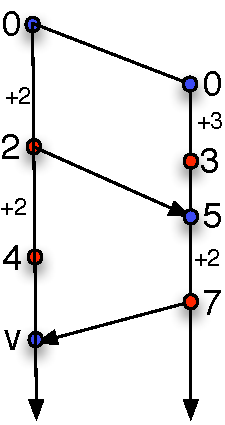
\includegraphics[scale=0.6]{Figures/merge-needs-lca}
\caption{This example of a grow-only counter illustrate why \C{merge}
needs a least common ancestor, and not just a common ancestor. Both 0
and 2 are common ancestors of 4 and 7, while 2 is their least common
ancestor (since $0 \preceq 2$). The result (v) of merging 4 and 7 is
11 (incorrect) if 0 is used as the common ancestor for merge, and 9
(correct, because 2+2+3+2 = 9) if 2 is used. }
\label{fig:merge-needs-lca}
\end{wrapfigure}
not be the case. With unrestrained branching and merging, there is no
bound on the number of LCAs a pair of versions can have.  For example,
in Fig.~\ref{fig:criss-cross-lcas}, the merge of 0 with 3 is preceded
by two ``criss-cross'' merges between their respective
branches\footnote{
  When discussing merges and LCAs, we often attribute the properties
  of latest versions on branches to the branches themselves.  For
  instance, when we say two branches merge, in fact their latest
  versions merge. Likewise, LCA of two branches means the LCA of their
  latest versions.
}
resulting in there being two LCAs (5 and 4) for 0 and 3. 
Multiple LCAs can occur even without criss-cross merges, as
demonstrated by Fig.~\ref{fig:external-lcas}. 
Concurrent versions with multiple LCAs do not lend themselves to
three-way merging. If such versions are latest on their respective
branches, they render the branches unmergeable (since  \C{lca} is no
longer a function) as demonstrated by examples in
Fig.~\ref{fig:many-lcas}. Note that for both the examples in
Fig.~\ref{fig:many-lcas}, no extension of the branching structure
can make the branches merge again. Thus the system is effectively
\emph{partitioned} permanently. This is clearly a problem. 

\begin{figure}[!t]
\centering
\subcaptionbox[] {\small
  In this example, 1 and 3 have two LCAs (3 and 4) a result of
  previous merges. The dotted circle denotes a virtual ancestor
  obtained by merging the two LCAs.
  \label{fig:criss-cross-lcas}
} [0.47\columnwidth] {
  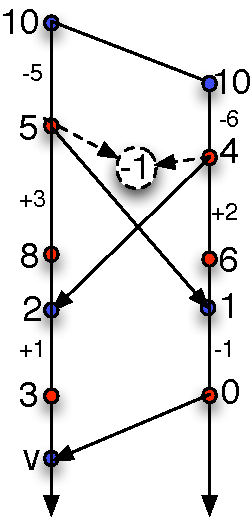
\includegraphics[scale=0.55]{Figures/2-LCAs}
}
\hfill
\subcaptionbox[] {\small
  In this example, versions $v_{13}$ and $v_{44}$ have two LCAs
  ($v_{22}$ and $v_{32}$)  despite there not being any previous merges
  between their respective branches.
  \label{fig:external-lcas}
} [0.47\columnwidth] {
  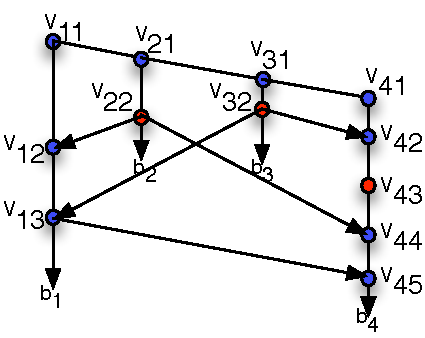
\includegraphics[scale=0.7]{Figures/2-external-LCAs}
}
\caption{Examples where two branches have more than one LCA, hence
cannot merge. }
\label{fig:many-lcas}
\end{figure}

The problem of multiple LCAs also arises in the context of source
control systems, which employ \emph{ad hoc} mechanisms to pave the way
for three-way merging.  GitHub~\cite{github}, for instance,
recursively merges LCAs to compute a virtual ancestor, which then
serves as the LCA for merging concurrent versions. This method is
demonstrated in the branching structure for a mergeable, replicated
counter as shown in Fig.~\ref{fig:criss-cross-lcas}, where LCAs 5 and
4 of 0 and 3 are merged (with their LCA being 10) to generate -1 as
the virtual LCA to merge 5 and 4. A major downside with this approach
is that it makes no guarantees on the relationship between the virtual
ancestor and its concurrent versions; the former may not even be a
legal ancestor of the latter as per the semantics of the data type.
For instance, suppose the integer type in
Fig.~\ref{fig:criss-cross-lcas} represents a bank account balance,
which is expected to disallows any activity on the account if the
balance is ever known to be less than zero.  From the perspective of
the library designer and its clients, there is no meaningful scenario
in which versions 3 and 0 can emerge from -1, since the only
transition allowed by the semantics from -1 is to itself.  Clearly,
\emph{ad hoc} mechanisms like this are error-prone and difficult to
apply in general.

Fortunately, unlike source control systems where branching structure
is entirely dictated by the user, \name abstracts away branching
structure from the programmer, and hence retains the ability to
manifest it in a way that it deems fit. In particular, \name solves
the problem of multiple LCAs by suitably constraining the branching
structure such that the problem never arises. The constraints are
imposed either implicitly, as a result of how operational semantics
defines an atomic step, or explicitly, by insisting that certain
conditions be met before merging a pair of versions
(\rulelabel{E-Pull-Wait}). Firstly, the operational semantics already
disables criss-cross merges since it only ever merges versions that
are latest on their respective branches. For instance, suppose
$v_{11}$ and $v_{21}$ are the latest versions on branches $b_1$ and
$b_2$, respectively. Merging $b_2$ into $b_1$ entails merging $v_{21}$
into $v_{11}$ to generate version $v_{12}$ on $b_1$.  Now, merging
$b_1$ into $b_2$ involves merging $v_{12}$, the latest version on
$b_1$, into $v_{21}$, but not $v_{11}$ into $v_{21}$, thus preempting
a criss-cross branching structure.

Secondly, we impose certain pre-conditions on the merging branches to
preempt the structure shown in Fig.~\ref{fig:external-lcas}. The
intuition is as follows: consider the branch $b_3$ at the instance of
merging $b_1$. Since it has already merged $b_2$, a version on $b_2$
($v_{21}$) could be a common ancestor for $b_3$ and some other branch
(call it $b$). Now, if $b_3$ merges $b_1$, same could be true of $b_3$
and $b_1$: a version on $b_1$ ($v_{11}$) could be a common ancestor
for $b_3$ and the other branch $v$. Since $v_{21}$ is also a common
ancestor for both the branches, and the ancestors are not ordered by
the ancestor relation, $b_3$ and $b$ end up with two LCAs. In
Fig.~\ref{fig:external-lcas}, the role of $b$ is played both by $b_1$
and $b_2$. We observe that this scenario can be prevented if, when
merging $b_1$, $b_3$ insists on an ancestor relation between the last
merged version ($v_{22}$) and the currently merging version.  We call
the last merged version of a branch its \emph{locus}. By maintaining a
total order of among locii of a branch $b$ as new versions are
created, we effectively guarantee the presence of a version (the
locus) that is lower than all the ancestors of the latest version on
$b$. Next, by requiring the locus to be an ancestor of the merging
version, we ensure that all the common ancestors have a single lowest
element, thus enforcing the uniqueness of the LCA.

We now formalize the intuitions described above via a series of
definitions that help us state the guarantees offered by the system.

\begin{definition} [\bfseries Internal and External Ancestors]
Given a branch $b$ and a version $v\in b$, an internal ancestor
($\preceq_i$) of $v$ is an ancestor from the same branch $b$. An
external ancestor ($\preceq_o$) of $v$ is an ancestor from a different
branch $b'\neq b$. 
\end{definition}

\begin{definition} [\bfseries Locus]
Given a branch $b$ and a version $v\in b$, locus ($v_o$) of $v$ is an
ancestor that is not an ancestor of any other external ancestor of
$v$. That is, $\under{H}{v_o \preceq v}$, and there does not exist a
$v_o' \not\in b$ such that $\under{H}{v_o' \preceq v}$ and
$\under{H}{v_o \preceq v_o'}$. We lift the notion of locus to the
level of branches by defining the locus of a branch as the locus of
its latest version.
\end{definition}

In a legal branching history, every version has a unique locus
(property follows from Def.~\ref{def:mergeability} below). Let
\emph{causal history} of a version be defined as the set of all
ancestors of that version. A locus ($v_o$) of a version ($v$) is
therefore the maximum element (lowest element in the ancestor
relation) of the causal history of $v$'s internal ancestor that was
the result of the last merge. We make use of this observation while
defining mergeability. 

\begin{definition} [\bfseries Mergeability]
\label{def:mergeability}
Given a history $H$, a version $v_1$ and a version $v_2$ that is not
an ancestor of $v_1$ under $H$, $v_2$ is mergeable into $v_1$ (denoted
$\under{H}{v_2 \mbleto v_1}$) if and only if the locus ($v_o$) of
$v_1$ is an ancestor of $v_2$, and no internal ancestor of $v_1$ that
is not also an ancestor of $v_o$ is an ancestor of $v_2$.    
\end{definition}

If $v_1$ and $v_2$ referred in the above definition are the latest
versions on their respective branches $b_1$ and $b_2$, we say $b_2$ is
mergeable into $b_1$, or more generally, $b_1$ and $b_2$ are
mergeable. The definition essentially requires all of $v_1$'s causal
history that preceeds its locus $v_o$ to be included in $v_2$'s causal
history, and none of $v_1$'s history that succeeds $v_o$ to be
included in $v_2$'s history. This allows us to view versions $v_1$ and
$v_2$ as having been independently evolved from a common causal
history whose maximum (w.r.t the ancestor relation) is the version
$v_o$. Consquently, $v_o$ becomes the LCA for $v_2$'s merge into
$v_1$. Generalizing this observation for the latest versions on
any two branches, we state the following theorem:

\begin{theorem} [\bfseries Unique LCA]
Every pair of branches in a legal history $H$, if mergeable as per
Def.~\ref{fig:mergeability}, have a unique least common ancestor.
\end{theorem}

While the definition of mergeability is sufficient to enforce
uniqueness of LCAs, it may hinder progress in the sense that there may
not exist a pair of branches in a legal history satisfying the
definition, thus making the progress impossible. The following theorem
asserts that this is not the case:

\begin{theorem} [\bfseries Progress]
In a legal branching history $H$ produced by the operational
semantics, if two branches, $b_i$ and $b_j$ are not mergeable (as per
Def.~\ref{def:mergeability}), then there exist a sequence of fork and
merge operations (between mergeable versions) that can be performed on
$H$ to yeild a new history $H'$, where $b_i$ and $b_j$ are mergeable.  
\end{theorem}

Proof is by the induction on the size of branching history. The
observation that the smallest history that is the union of causal
histories of two unmergeable versions (call them $v_i$ and $v_j$) is
smaller than the history that includes the unmergeable versions. Since
causal histories have maximum versions (respective locii), which, by
inductive hypothesis, can be made mergeable, we merge them to yeild a
new version $v$ that is the maximum of the causal histories of both
$v_i$ and $v_j$. If $v_i$ and $v_j$ are the latest versions on their
respective branches, the branches are now mergeable.  

% Observe that $v$ and $v_i$ are mergeable (with
% $v_i$'s locus as the LCA), and so do $v$ and $v_j$. If $v_i$ and $v_j$
% are the latest versions on their respective branches, then merging $v$
% into $v_i$ and $v$ into $v_j$ makes $v$ the locus of both the
% branches, thus making them mergeable again. 

% \begin{theorem} [\bfseries Progress and Eventual Convergence] Given a
% legal branching history $H$, and a program $p$, where every thread
% expression in $p$ is a \C{pull}, there exist a series of reduction steps
% that reduce $p; H$ to $p'; H'$, where every thread expression in $p$
% is the same value $v$.
% \end{theorem}


\subsection{System Model}

